\begin{frame}[t,fragile]{自動微分(後退モード)}
  \begin{itemize}
    %\setlength{\itemsep}{1em}
  \item 後退モード(Backward mode)・トップダウン型(Top-down)計算
  \item まず、下から順に $v_1, v_2, \cdots$ の値、および各基本演算における微分係数をもとめておく
    \begin{itemize}
    \item $v_1 \leftarrow \exp(x_2) = 1$, $d_{v_1,x_2} \leftarrow \frac{\partial v_1}{\partial x_2} = \exp(x_2) = 1$
    \item $v_2 \leftarrow x_1 - v_1 = 1$, $d_{v_2,x_1} \leftarrow \frac{\partial v_2}{\partial x_1} = 1$, $d_{v_2,v_1} \leftarrow \frac{\partial v_2}{\partial v_1} = -v_1 = -1$,
    \item $v_3 \leftarrow v_1 \times x_3 = 1$, $d_{v_3,v_1} \leftarrow \frac{\partial v_3}{\partial v_1} = x_3 = 1$, $d_{v_3,x_3} \leftarrow \frac{\partial v_3}{\partial x_3} = v_1 = 1$
    \item $v_4 \leftarrow v_2 \times v_3 = 1$
    \item $d_{v_4,v_2} \leftarrow \frac{\partial v_4}{\partial v_2} = v_3 = 1$
    \item $d_{v_4,v_3} \leftarrow \frac{\partial v_4}{\partial v_3} = v_2 = 1$
    \item $v_5 \leftarrow v_3 + 1 = 2$
    \item $d_{v_5,v_3} \leftarrow \frac{\partial v_5}{\partial v_3} = 1$
    \item $f \leftarrow v_4 / v_5 = 1/2$
    \item $d_{f,v_4} \leftarrow \frac{\partial f}{\partial v_4} = \frac{1}{v_5} = \frac{1}{2}$
    \item $d_{f,v_5} \leftarrow \frac{\partial f}{\partial v_5} = -\frac{v_4}{(v_5)^2} = -\frac{1}{4}$
    \end{itemize}
    \vspace*{-9em} \hfill \resizebox{.3\textwidth}{!}{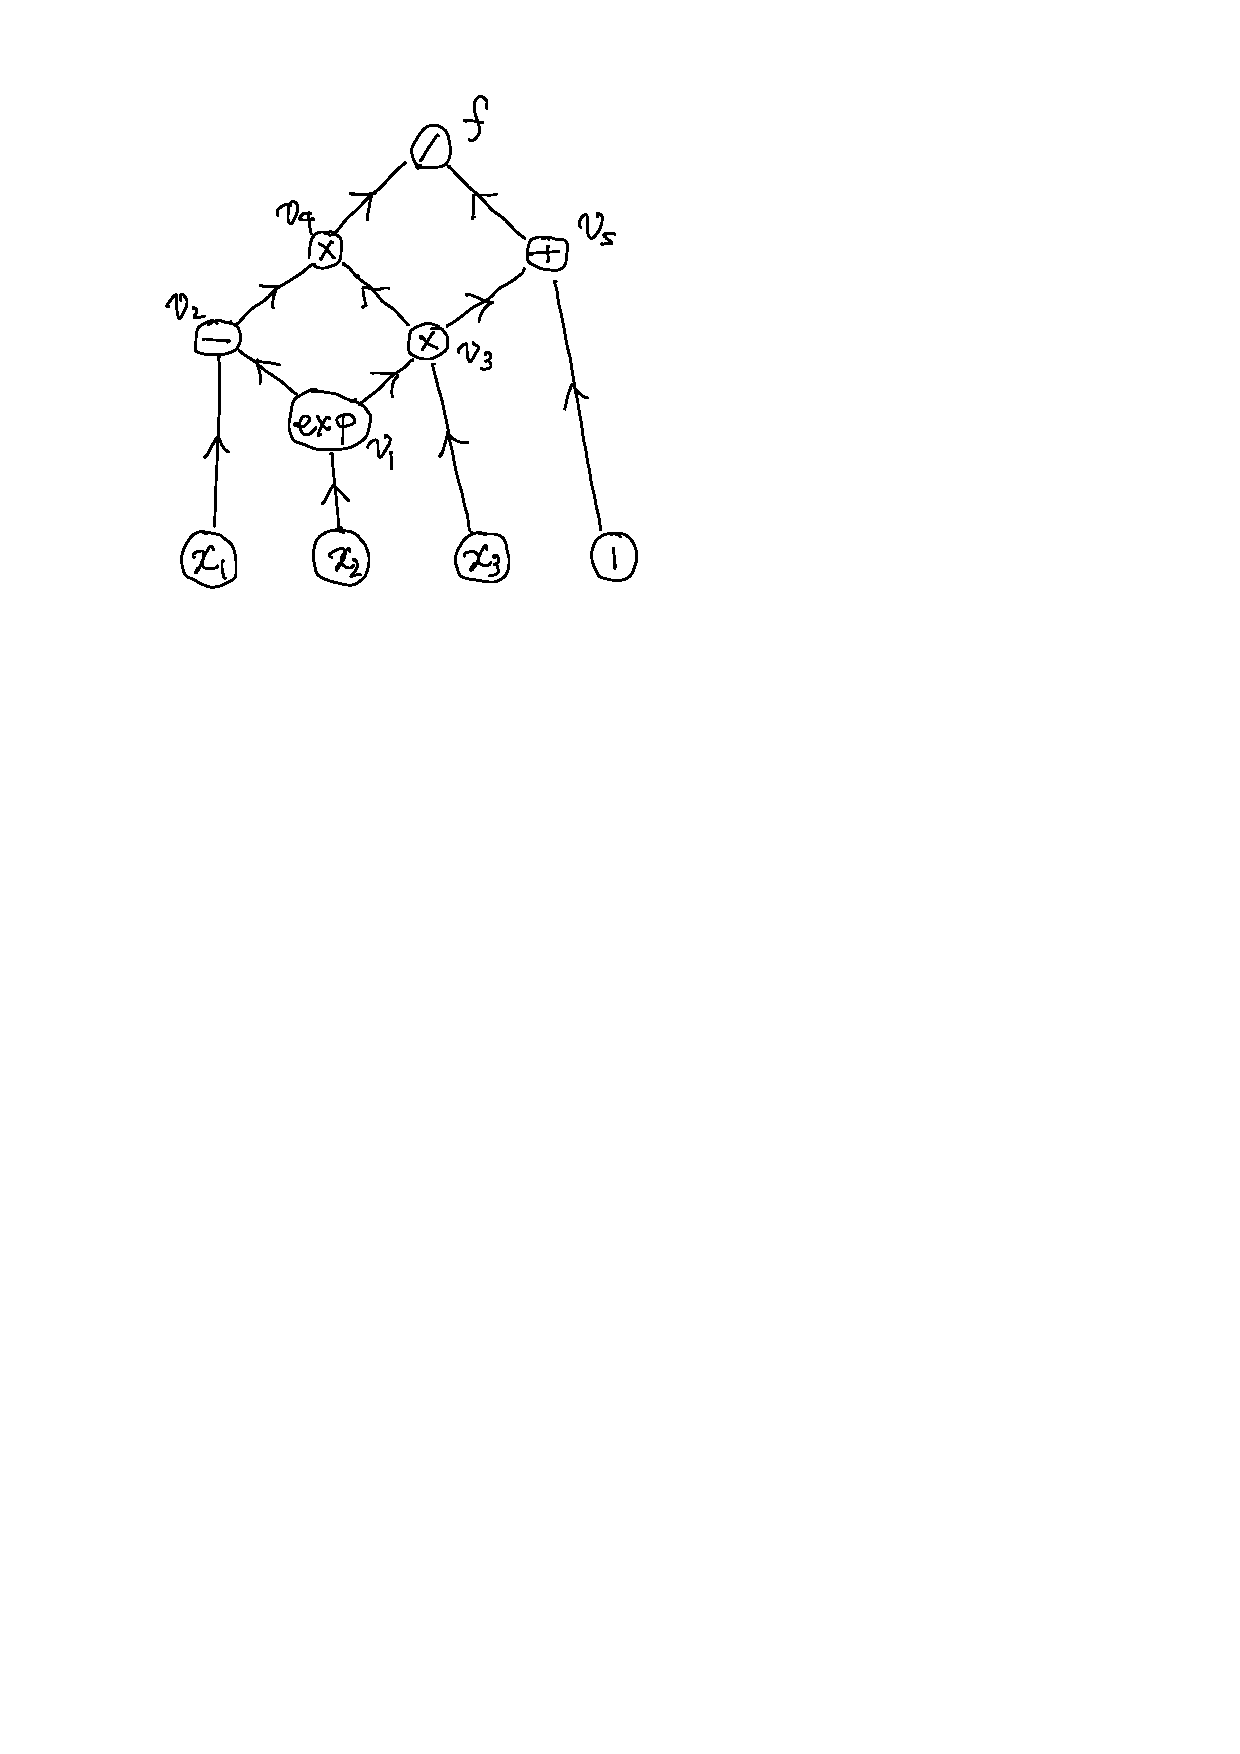
\includegraphics{image/compgraph.pdf}}
  \end{itemize}
\end{frame}
